\documentclass{article}
\usepackage[utf8]{inputenc}
\usepackage{amsmath}
\usepackage{amsfonts}
\usepackage{amssymb}
\usepackage{graphicx}
\newtheorem{theorem}{Theorem}

\title{Multivariate statistical dependence measure based on characteristic functions}
\author{povilas.daniusis, povilasd@neurotechnology.com}
\date{November 2021}

\begin{document}
\maketitle

\begin{abstract}
    In this paper we propose  multivariate statistical dependence measure based on difference between joint and marginal characteristic functions. We discuss simulated examples, and applications for feature selection/extraction, causal inference and conduct corresponding experiments with diverse collection of multivariate data sets.
\end{abstract}
\section{Introduction}
\section{Previous work}

\section{Proposed Method}

We will derive independence measure relying on property of characteristic functions (also known as Kac theorem~\cite{KacTheorem}), that independence of two random vectors $X \in R^{d_{x}}$ and $Y \in R^{d_{y}}$ is equivalent to $\forall \alpha \in R^{d_x}, \beta \in R^{d_y} $, \begin{equation}
\mathbb{E}_{X,Y} e^{i <\alpha, X> + i <\beta, Y>} = \mathbb{E}_{X} e^{i <\alpha, X>} \mathbb{E}_{Y} e^{i <\beta, Y>},
\end{equation}
where $i = \sqrt{-1}$, $d_{x}$ and $d_{y}$ are dimensions of $X$ and $Y$, respectively.

\noindent This motivates the construction of a novel statistical dependence measure, which we further refer to as Kac independence measure (KacIM):
\begin{equation}
\label{eq:kim}
    \kappa(X,Y) = \max_{\alpha, \beta} \vert \mathbb{E}_{X,Y} e^{i <\alpha, X> + i <\beta, Y>} -\mathbb{E}_{X} e^{i <\alpha, X>} \mathbb{E}_{Y} e^{i <\beta, Y>} \vert
\end{equation}

\noindent It is easy to see that $0 \leq \kappa(X,Y) \leq 1$, $\kappa(X,Y) = \kappa(Y,X)$. 

\subsection{Estimation}

Having i.i.d. data $(x_{j}, y_{j})$, $j = 1,2,...,n$ an empirical estimator of KacIM~\eqref{eq:kim} is defined via corresponding empirical characteristic functions:
\begin{equation}
\label{eq:estimator}
    \hat{\kappa}(X,Y) = \max_{\|\alpha\| = \|\beta\| = 1} \vert \frac{1}{n} \sum_{j=1}^{n} e^{i(<\alpha, x_{j}> + <\beta, y_{j}>) } - \frac{1}{n^2} \sum_{j=1}^{n} e^{i <\alpha, x_{j}>}\sum_{k=1}^{n} e^{i<\beta, y_{k}>}\vert.
\end{equation}

\noindent Empirical estimator also admits $0 \leq \hat{\kappa}(X,Y) \leq 1$. Normalisation of parameters $\alpha$ and $\beta$ on to unit sphere is included due to stability issues. The  estimator~\eqref{eq:estimator} can be calculated by using gradient ascend.

\section{Experiments}
Dependence measures have board area of applications. For example, regularization~\cite{?,?}, feature selection and extraction~\cite{?}, information bottleneck methods \cite{?}, causal inference~\cite{?}, among others. Further we will reformulate some key ideas in these topics for KacIM, and experimentally investigate corresponding empirical scenarios.


\subsection{Generated data}

We begin with simple example, which demonstrates the efficiency of KacIM for simulated multivariate data with additive and multiplicative noise.

\begin{figure}[t]
\label{fig:experiments_simulation}
\centering
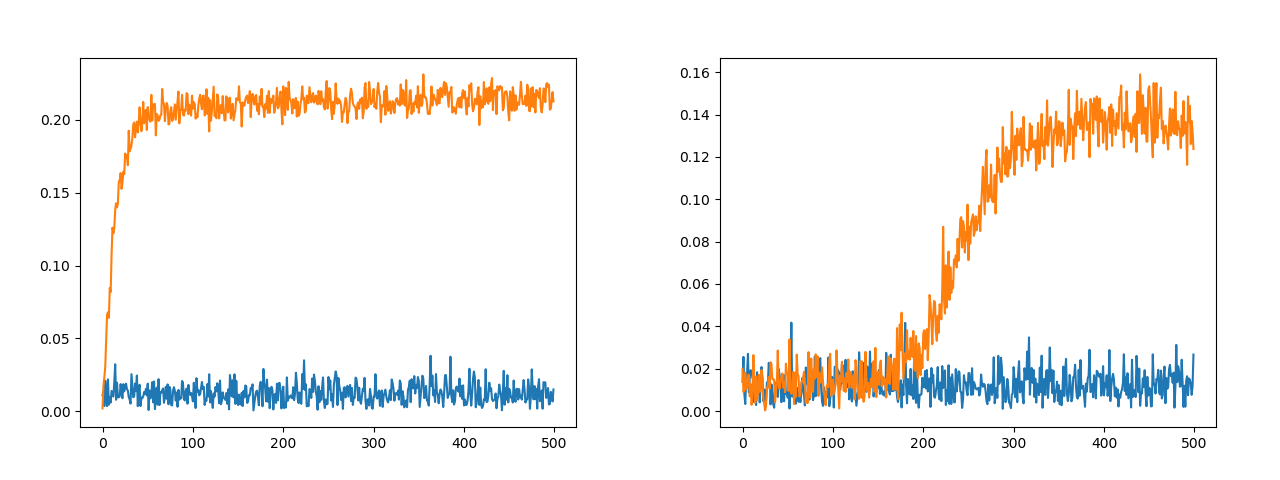
\includegraphics[scale=0.25]{./out.png}
\caption{Dependence detection in additive (left) and multiplicative (right) noise scenario.}
\end{figure}

In Figure~\ref{fig:experiments_simulation} reflects KacIM values during iterative adaptation ($500$ iterations). In the case of independent data, both $x_{i}$ and $y_{i}$ ($d_{x} = 1024$, $d_{y} = 32$) are sampled from gaussian distribution, independently. In the case of dependent data, an additive noise (left graph) and multiplicative noise (right graph), the dependent variable is generated according to $y_{i} = sin(P x_{i}) + cos(P x_{i}) + \lambda \epsilon_{i}$ ($\lambda = 0.15$) and $y_{i} = (sin(P x_{i}) + cos(P x_{i})) \epsilon_{i}$, respectively, where $P$ is $d_{x} \times d_{y}$ random projection matrix, $\epsilon_{i} \sim N(0,1)$ and $\epsilon_{i} \perp x_{i}$.

When data is independent (blue graph), both in additive and multiplicative cases, due to independence, estimator~\eqref{eq:estimator} is resistant to maximization, and oscillates near zero. On the other hand, when data is not independent (orange graph), the condition of Kac theorem is violated and maximization of estimator~\eqref{eq:estimator} is possible.

\subsection{Influence of noise level $\lambda$ to KacIM estimator value}
In this simulation we use the same additive noise setting as in previous paragraph, but evaluate all noise levels $\lambda \in [0.0, 2.4]$, with step $0.1$.
Figure~\ref{fig:experiments_noise_level_effect} empirically shows that value of KacIM correlates with noise level, and therefore the proposed measure is able not only to detect whether independence is present, but also to quantitatively evaluate it, which enables to use KacIM to derive cost functions for vairous other learning-based algorithms. %This continuity property is useful for various applications (e.g. using KacIM as the basis of cost function in various algorithms).

\begin{figure}[t]
\label{fig:experiments_noise_level_effect}
\centering
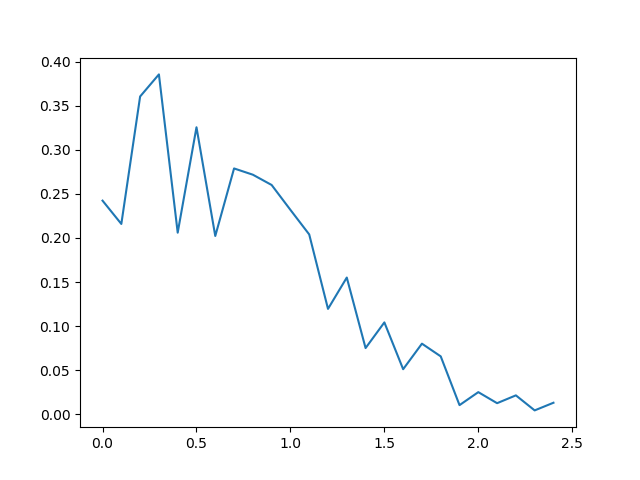
\includegraphics[scale=0.50]{./noise_level_effect_to_kacim.png}
\caption{Noise level ($x$ axis) vs final iteration KacIM value ($y$ axis). KacIM values for larger noise levels saturates to the level similar to its final values.}
\end{figure}



\subsection{Feature Extraction}

We conduct linear feature extraction by seeking 

\begin{equation}
\label{eq:kim_feature_extraction}    
W^{*} = arg \max_{W} \kappa(Wx, y).
\end{equation}


%\begin{equation}
%\label{eq:kim_feature_extraction1}    
%w_{t}^{*} = arg \max_{W} \frac{\kappa(w_{t}^{T}x, y)}{\kappa(w_{t}^{T}x, W_{t}x)}.
%\end{equation}

\noindent Afterwards, feature extraction is conducted by $f = W^{*}x$ and $k$-nearest neighbor classification with Euclidean distance is performed, comparing unmodified inputs $x$ and features of all possible dimensions up to $d_{x}$.

\section{Discussion} 


%\subsection{KacIM for information bottleneck}
%\subsection{Canonical component analysis, independent component analysis}
%\subsection{Causal inference}
%\subsection{Electroencephalography (?)}
%\section{Notes}
%Compare with  mutual information.

\begin{thebibliography}{}
\bibitem{KacTheorem} David Applebaum, B.V. Rajarama Bhat, Johan Kustermans, J. Martin Lindsay, Michael Schuermann, Uwe Franz: Quantum Independent Increment Processes I: From Classical Probability to Quantum Stochastic Calculus

\end{thebibliography}
\end{document}
